\documentclass[11pt]{scrartcl}
\usepackage[T1]{fontenc}
\usepackage[a4paper, left=3cm, right=2cm, top=2cm, bottom=2cm]{geometry}
\usepackage[activate]{pdfcprot}
\usepackage[ngerman]{babel}
\usepackage[parfill]{parskip}
\usepackage[utf8]{inputenc}
\usepackage{kurier}
\usepackage{amsmath}
\usepackage{amssymb}
\usepackage{xcolor}
\usepackage{epstopdf}
\usepackage{txfonts}
\usepackage{fancyhdr}
\usepackage{graphicx}
\usepackage{prettyref}
\usepackage{hyperref}
\usepackage{eurosym}
\usepackage{setspace}
\usepackage{units}
\usepackage{eso-pic,graphicx}
\usepackage{icomma}
\usepackage{pdfpages}

\definecolor{darkblue}{rgb}{0,0,.5}
\hypersetup{pdftex=true, colorlinks=true, breaklinks=false, linkcolor=black, menucolor=black, pagecolor=black, urlcolor=darkblue}



\setlength{\columnsep}{2cm}


\newcommand{\arcsinh}{\mathrm{arcsinh}}
\newcommand{\asinh}{\mathrm{arcsinh}}
\newcommand{\ergebnis}{\textcolor{red}{\mathrm{Ergebnis}}}
\newcommand{\fehlt}{\textcolor{red}{Hier fehlen noch Inhalte.}}
\newcommand{\betanotice}{\textcolor{red}{Diese Aufgaben sind noch nicht in der Übung kontrolliert worden. Es sind lediglich meine Überlegungen und Lösungsansätze zu den Aufgaben. Es können Fehler enthalten sein!!! Das Dokument wird fortwährend aktualisiert und erst wenn das \textcolor{black}{beta} aus dem Dateinamen verschwindet ist es endgültig.}}
\newcommand{\half}{\frac{1}{2}}
\renewcommand{\d}{\, \mathrm d}
\newcommand{\punkte}{\textcolor{white}{xxxxx}}
\newcommand{\p}{\, \partial}
\newcommand{\dd}[1]{\item[#1] \hfill \\}

\renewcommand{\familydefault}{\sfdefault}
\renewcommand\thesection{}
\renewcommand\thesubsection{}
\renewcommand\thesubsubsection{}


\newcommand{\themodul}{Optische Technologie}
\newcommand{\thetutor}{Prof. Rateike}
\newcommand{\theuebung}{Übung 2}

\pagestyle{fancy}
\fancyhead[L]{\footnotesize{C. Hansen}}
\chead{\thepage}
\rhead{}
\lfoot{}
\cfoot{}
\rfoot{}

\title{\themodul{}, \theuebung{}, \thetutor}


\author{Christoph Hansen \\ {\small \href{mailto:chris@university-material.de}{chris@university-material.de}} }

\date{}


\begin{document}

\maketitle

Dieser Text ist unter dieser \href{http://creativecommons.org/licenses/by-nc-sa/4.0/}{Creative Commons} Lizenz veröffentlicht.

\textcolor{red}{Ich erhebe keinen Anspruch auf Vollständigkeit oder Richtigkeit. Falls ihr Fehler findet oder etwas fehlt, dann meldet euch bitte über den Emailkontakt.}

\tableofcontents


\newpage



\section{Aufgabe 1}


\subsection*{a)}

Für die innere Transmission müssen wir zunächst $\tau$ ausrechnen:

\begin{align*}
\tau &= e^{-Kd} = e^{- 10 \cdot 0,1} = e^{-1} = 0,37
\intertext{Das können wir nun in die Formel für die Transmission einsetzen:}
T &\approx \left( 1 - R \right)^2 \cdot \tau = 0,96^2 \cdot 0,37 = 0,34
\end{align*}


\subsection*{b)}

Mit der exakten Formel kommen wir auf:

\begin{align*}
T &= \frac{\left( 1 - R \right)^2 \cdot \tau}{1 - \left( R \tau \right)^2} = \frac{0,34}{1 - \left( 0,04 \cdot 0,37 \right)^2} = 0,34
\end{align*}

Zwischen Näherung und genauem Wert gibt es in diesem Fall keinen Unterschied.


\section{Aufgabe 2}

Die Dicke geht exponentiell in die innere Transmission ein:

\begin{align*}
e^{- K \cdot 2d} = \left( e^{-Kd} \right)^2 \\
e^{- K \cdot 3d} = \left( e^{-Kd} \right)^3
\end{align*}

\newpage

\section{Aufgabe 3}

\begin{figure}[h]
	\centering
	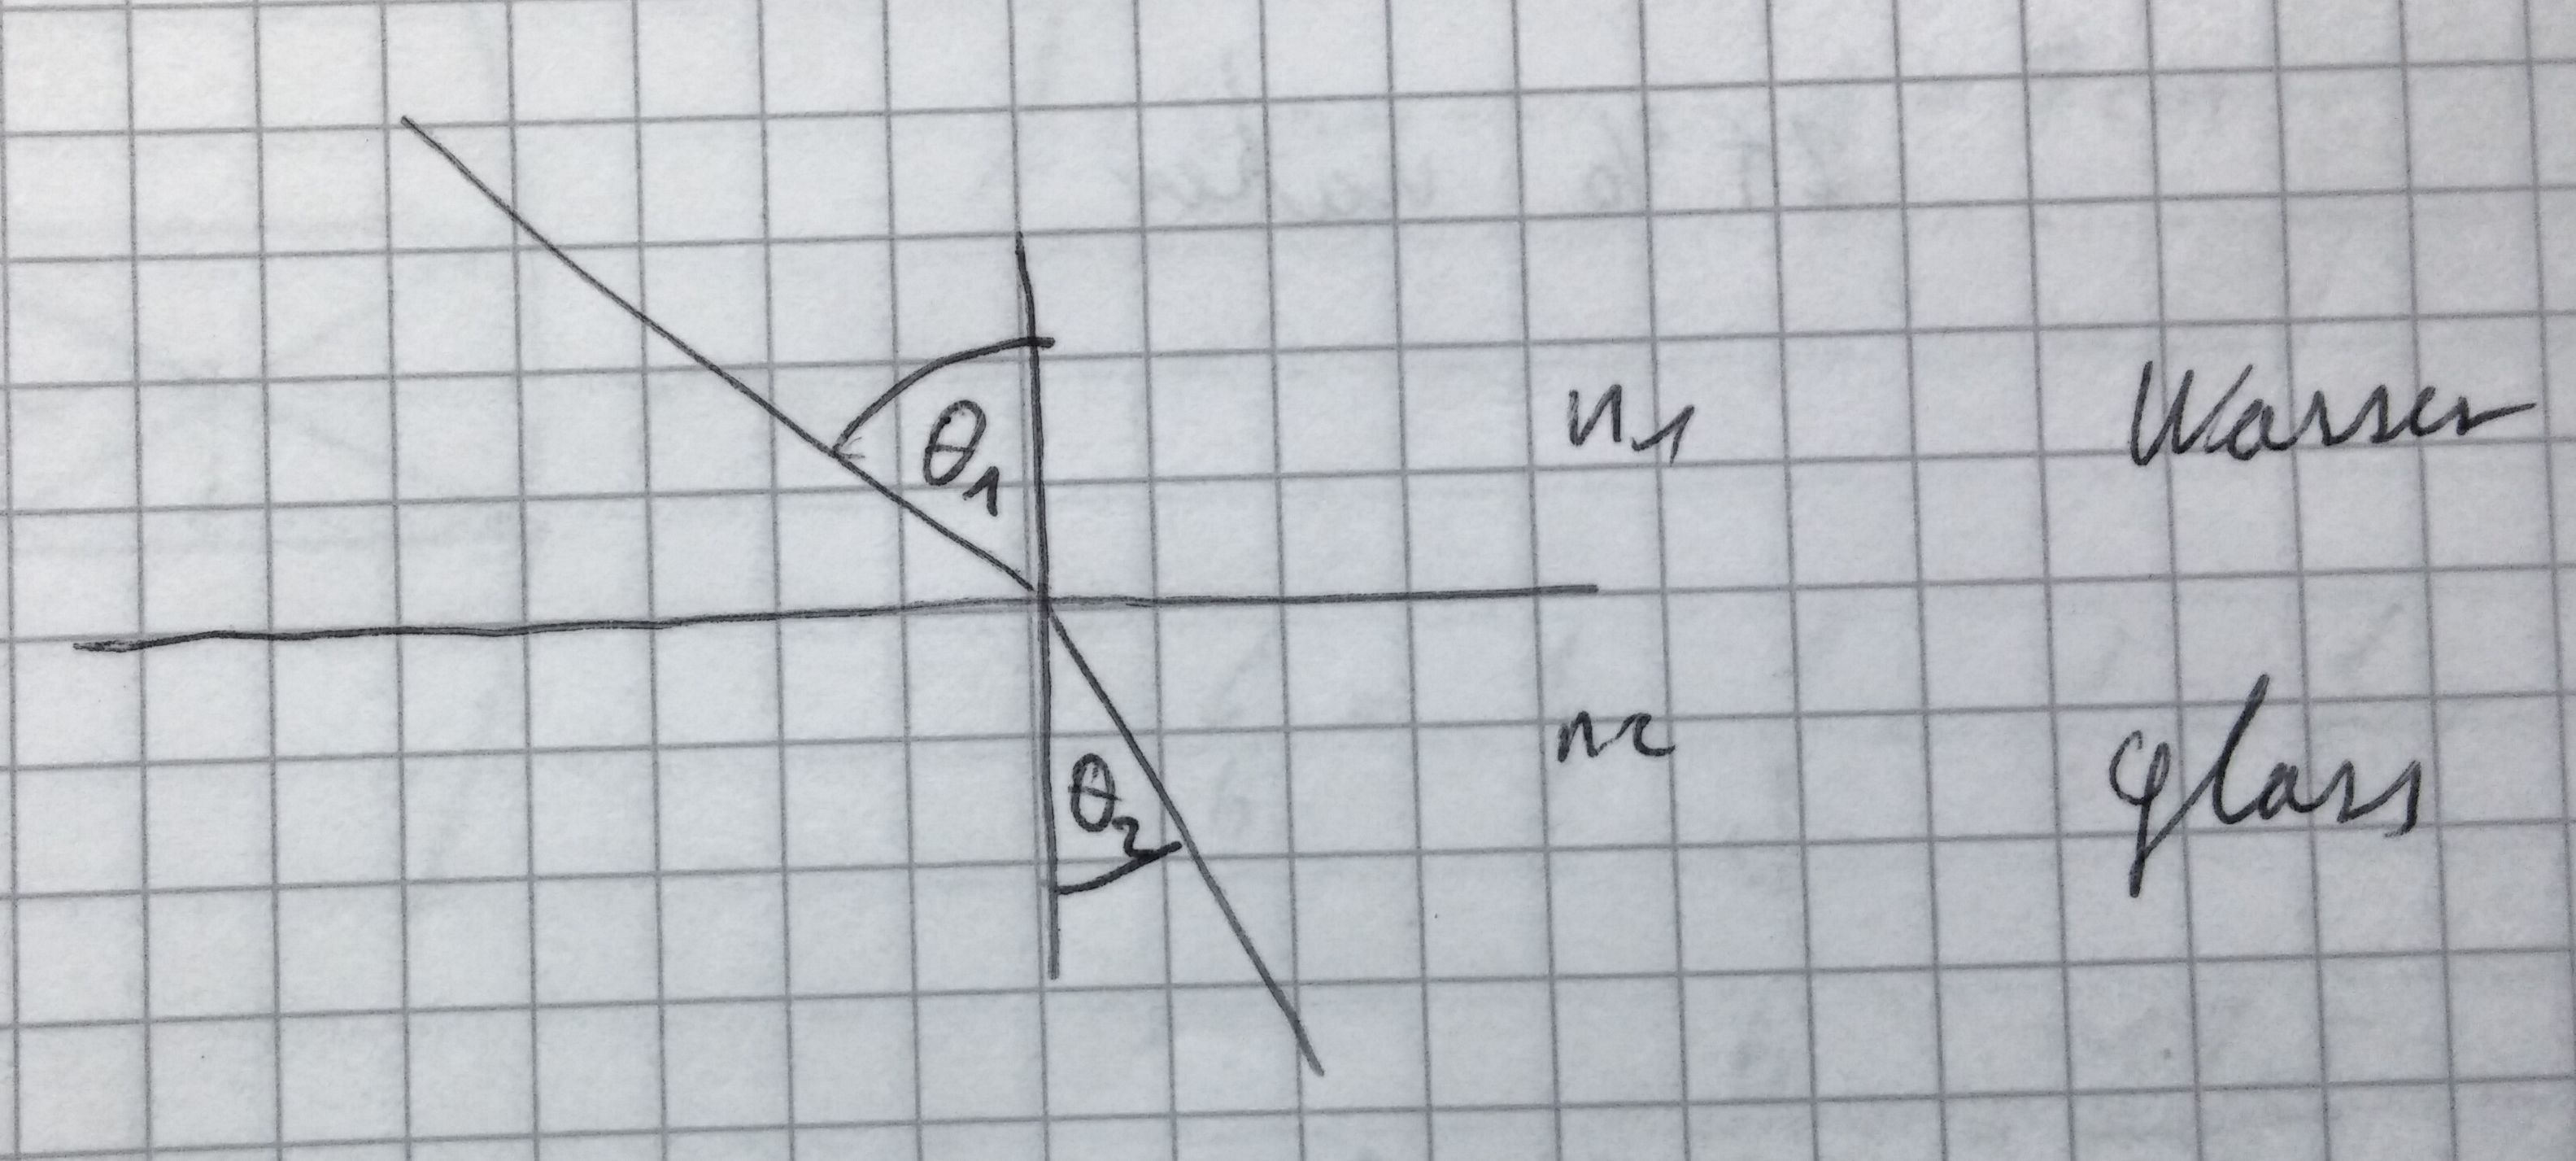
\includegraphics[scale=0.15]{A3_1.jpg}
\end{figure}


Der Unterschied liegt wie im Bild zu sehen in der Anzahl der Reflexionen.


\section{Aufgabe 4}

Die allgemeine Formel für Oberflächenreflexion ist:

\begin{align*}
R &= \left( \frac{n - 1}{n + 1} \right)^2
\intertext{Wir suchen uns aus einer Tabelle die entsprechenden Werte heraus und setzen ein:}
R_{BK7} &= \left( \frac{1,52 - 1}{1,52 + 1} \right)^2 = 0,042 \\
R_{SF11} &= \left( \frac{1,78 - 1}{1,78 + 1} \right)^2 = 0,079
\end{align*}


\section{Aufgabe 5}

Durch angucken in einer Tabelle wissen wir das hier nur Calciumfluorid und Fused Silica geeignet sind.


\section{Aufgabe 6}

Hier ist wiederum Calciumfluorid und grade so noch Saphir zu gebrauchen.


\section{Aufgabe 7}

Wir haben dabei hohe Reflexionsverluste.


\section{Aufgabe 8}

\subsection*{a)}

\begin{align*}
R &= \left( \frac{4,028 - 1}{4,028 + 1} \right)^2 = 0,36
\end{align*}

\subsection*{b)}

\begin{align*}
n_{AR} &= \sqrt{n_S} = \sqrt{4,028} \approx 2
\end{align*}

\subsection*{c)}

\begin{align*}
d &= \frac{\lambda}{4 \cdot n} = \frac{10,6 \cdot 10^{-6}}{4 \cdot 4,028} \approx \frac{10,6 \cdot 10^{-6}}{16} = \unit[0,66]{\mu m}
\end{align*}






\end{document}